% Created 2011-01-07 Пт. 09:45
\documentclass[12pt, russian, oneside, article]{ncc}
\usepackage[utf8]{inputenc}
\usepackage[T1]{fontenc}
\usepackage{fixltx2e}
\usepackage{graphicx}
\usepackage{longtable}
\usepackage{float}
\usepackage{wrapfig}
\usepackage{soul}
\usepackage{textcomp}
\usepackage{marvosym}
\usepackage{wasysym}
\usepackage{latexsym}
\usepackage{amssymb}
\usepackage{hyperref}
\tolerance=1000
\usepackage[math]{pscyr}
\usepackage{indentfirst}
\providecommand{\alert}[1]{\textbf{#1}}
\begin{document}



\title{Системы и сети передачи информации}
\author{Максим Захаров}
\date{07 Январь 2011}
\maketitle

\setcounter{tocdepth}{3}
\tableofcontents
\vspace*{1cm}


\href{file:///home/maxim/Documents/Git/lectures/index.org}{На главную} | \href{file:///home/maxim/Documents/Git/lectures/other/SiSPI_Lectures.pdf}{Скачать в PDF}

\section{Логическая многоуровневая организация ЗТКС}
\label{sec-1}


Организация ТКС должна удовлетворять следующим требованиям.
\begin{enumerate}
\item Открытость. Возможность подключения дополнительных узлов, абонентов, линий связи без изменения существующих технических и программных средств.
\item Гибкость. Сохранение работоспособности при изменении структуры системы (при выходе из строя отдельных компонентов).
\item Эффективность. Обеспечение требуемого качества обслуживания абонентов при минимальных затратах.
\end{enumerate}
  
\subsection{Процессы}
\label{sec-1_1}


\begin{enumerate}
\item Прикладные процессы выполняют задачи пользователя.
\item Системные выполняют вспомогательные функции, обеспечивающие функционирование прикладных процессов.
\end{enumerate}

Ввод и вывод данных, необходимых процессу, производится \textbf{сообщениями} через программно-организованные логические точки, называемые порты.
\subsection{Модель взаимодействия открытых систем}
\label{sec-1_2}


В 1978 году международная организация по стандартизации ISO ввела новую модель стандартов, которая получила название ``модель взаимодействия открытых систем'' --- ISO/OSI.

Данная модель обладала следующими особенностями:
\begin{enumerate}
\item Является стандартом в передаче данных, позволяющим системам различных производителей устанавливать сетевые соединения.
\item Состоит из 7 уровней со специфическим набором функций и включает описание межуровневых интерфейсов.
\item Определяет набор протоколов и интерфейсов для каждого уровня.
\end{enumerate}
\subsection{Функции уровней модели OSI}
\label{sec-1_3}
\subsubsection{Физический уровень}
\label{sec-1_3_1}


Контролирует путь, по которому поток битов данных передаётся и принимается из физической среды передачи. Он определяет электрический, оптический, электромагнитный и механический интерфейс для передающей среды. Он принимает сигналы из среды передачи и преобразует их в цифровые данные, которые используют все вышележащие уровни.
\subsubsection{Канальный уровень}
\label{sec-1_3_2}


Обеспечивает безошибочную передачу кадров данных между системами через физический уровень.

Выполняет следующие функции:
\begin{enumerate}
\item Установление и разрыв связи между двумя системами, определёнными адресами их сетевых адаптеров (MAC-адрес).
\item Последовательная передача и приём кадров.
\item Проверка правильности данных в принятых кадрах и подтверждение успешного приёма кадров (функция квитирования).
\item Ожидание подтверждения приёма кадра; инициализация повторной передачи кадра; разрешение вопросов, связанных с дублированием кадров.
\item Определение границ кадров.
\item Управление доступом в передающую среду путём определения оптимального момента начала передачи.
\item Анализ пункта назначения принятого кадра.
\end{enumerate}

Протоколы канального уровня называются протоколами прямой передачи или пиринговые протоколы. Они устанавливают соединения только с непосредственными соседями в сети, с которыми у них общая среда передачи.
\subsubsection{Сетевой уровень}
\label{sec-1_3_3}


Контролирует работу сети. Он определяет какой физический путь должны пройти данные исходя из логического адреса получателя. Протокольная единица --- пакет.

Функции:
\begin{enumerate}
\item Передача пакета маршрутизатору в том случае, если сетевой адрес пункта назначения не находится в той же подсети, что и отправитель.
\item Установление однозначной связи логического адреса на сетевом уровне и физического адреса на канальном --- ARP.
\item Возможность использования альтернативного маршрута в случае отказа основного маршрутизатора.
\item Управление фрагментацией пакетов.
\item Возможность учёта количества переданных пакетов для работы биллинговой системы.
\end{enumerate}
\subsubsection{Транспортный уровень}
\label{sec-1_3_4}


Протокольная единица --- сегмент/дейтаграмма.

Гарантирует доставку сообщений в том порядке, в каком они были посланы. Гарантирует отсутствие потерь и дублирования информации.

Функции:
\begin{enumerate}
\item Приём сообщений с вышележащего уровня и, при необходимости, разбивка их на сегменты.
\item Обеспечение надёжной и гарантированной доставки сообщений и подтверждение успешного приёма.
\item Управление передающей системой с помощью команд на прекращение передачи, если приёмные буферы заполнены.
\item Мультиплексирование нескольких потоков сообщений между процессами в одном логическом соединении.
\end{enumerate}
\subsubsection{Сеансовый уровень.}
\label{sec-1_3_5}


Протокольная единица --- сообщение.

Устанавливает связь или сеанс между процессами, работающими в различных системах, и поддерживает обмен данных в режиме сообщений

Функции:
\begin{enumerate}
\item Позволяет прикладным процессам регистрировать уникальные адреса (номера портов).
\item Установление, мониторинг и окончание сеанса по виртуальной сети.
\item Определение границ сообщений с помощью информации из заголовка.
\end{enumerate}
\subsubsection{Уровень представления данных}
\label{sec-1_3_6}


Используют данные пользователя.

Служат транслятором данных, передаваемых по сети. Преобразуют данных из формата приложения в общепринятый формат.

Функции:
\begin{enumerate}
\item Трансляция символов в коды.
\item Конвертирование данных.
\item Сжатие данных.
\item Шифрование.
\end{enumerate}
\subsubsection{Прикладной уровень}
\label{sec-1_3_7}


Предоставляет пользователю доступ к сетевому сервису. Сколько сервисов, столько и функций.
\subsection{Интерфейс и структура сообщений}
\label{sec-1_4}

  
Интерфейс определяет структуру данных и алгоритм обмена данными между соседними уровнями одной системы.

Многоуровневая организация системы для эффективного управления требует модификации сообщений на каждом уровне. Модификация заключается в добавлении заголовка и концевика, в которых содержится информация, необходимая для управления.

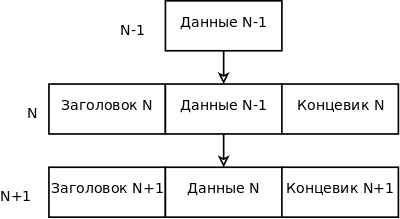
\includegraphics[width=0.7\textwidth]{images/SiSPI/mess_strucr.png}
\subsection{Протоколы}
\label{sec-1_5}


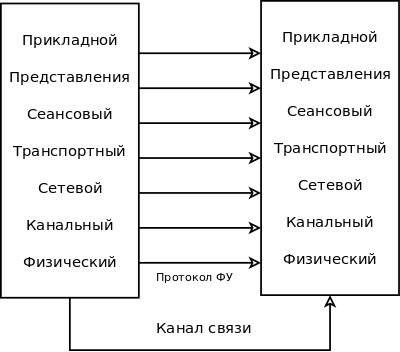
\includegraphics[width=0.7\textwidth]{images/SiSPI/protocol.png}

Совокупность правил взаимодействия процессов одноимённых уровней разных систем называется \emph{протокол}.
\section{Топологии сетей}
\label{sec-2}


\emph{Топология} --- геометрическая форма или физическая связанность сети.
\subsection{Шина (Bus)}
\label{sec-2_1}


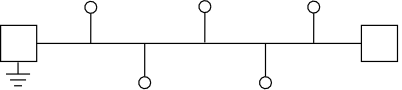
\includegraphics[width=0.7\textwidth]{images/SiSPI/bus.png}

Преимущества:
\begin{itemize}
\item гибкость и открытость;
\item простота управления.
\end{itemize}

Недостатки:
\begin{itemize}
\item в случае отказа канала вся сеть не функционирует;
\item пропускная способность делится между всеми абонентами сети;
\item длина шина ограничена мощностью сигнала;
\item если два узла начинают передавать одновременно, то возникает ошибка.
\end{itemize}
\subsection{Кольцо (Ring)}
\label{sec-2_2}


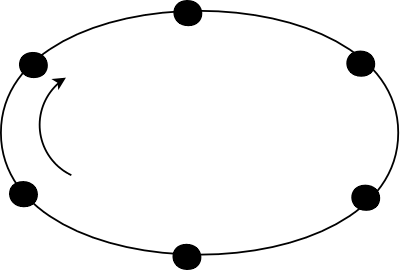
\includegraphics[width=0.7\textwidth]{images/SiSPI/ring.png}

Преимущества:
\begin{itemize}
\item сигнал усиливается каждым промежуточным узлом, т. е. размер кольца может быть очень большим;
\item чёткий географический приоритет между станциями;
\item эффективное использование пропускной способности;
\item невозможность коллизий или столкновений.
\end{itemize}

Недостатки:
\begin{itemize}
\item выход из строя любого абонента приведёт к неработоспособности сети;
\item низкая открытость сети.
\end{itemize}
\subsection{Звезда (Star)}
\label{sec-2_3}


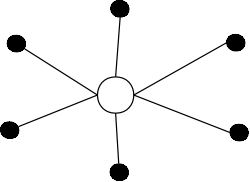
\includegraphics[width=0.7\textwidth]{images/SiSPI/star.png}

Достоинства:
\begin{itemize}
\item выход из строя абонента или кабеля этого абонента не влияет на работоспособность сети (лёгкая локализация неисправностей сети);
\item централизованное управление, отсутствие перегрузок и конфликтов.
\end{itemize}

Недостатки:
\begin{itemize}
\item требования к центральному узлу повышены и по надёжности и по работоспособности;
\item количество абонентов в сети ограничено.
\end{itemize}
\subsection{Дерево (Tree)}
\label{sec-2_4}


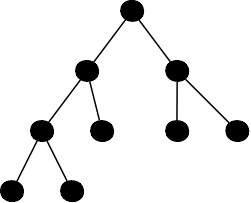
\includegraphics[width=0.7\textwidth]{images/SiSPI/tree.png}

Разновидность топологии ``звезда''. По такой топологии обычно реализуется управление в больших сетях.
\subsection{Сеть (Network)}
\label{sec-2_5}


Представляет собой древовидную топологию, в которой добавлены резервные или альтернативные связи до отдельных узлов.
\section{Методы коммутации}
\label{sec-3}


По способам передачи данных различают сети с коммутацией каналов, с коммутацией сообщений и с коммутацией пакетов.
\subsection{Сеть с коммутацией каналов}
\label{sec-3_1}


Рисунок 7

Для передачи данных необходимо установление между пользователями прямого физического соединения.

Достоинства:
\begin{itemize}
\item работа в режиме реального времени и полностью используют пропускную способность всех каналов;
\item эффективна при передаче больших объёмов данных.
\end{itemize}

Недостатки:
\begin{itemize}
\item система работает с отказами, т. е. необходимо дожидаться освобождения линии связи;
\item невозможность приоритетной передачи данных;
\item неэффективна при передаче небольших объёмов данных.
\end{itemize}
\subsection{Сеть с коммутацией сообщений}
\label{sec-3_2}


Рисунок 8

Сообщение снабжается заголовком, в котором указывается получатель и передаётся последовательно от узла коммутации к узлу.

Достоинства:
\begin{itemize}
\item нет сигналов ``занято'' или отказов сети;
\item возможность приоритетной передачи;
\end{itemize}

Недостатки:
\begin{itemize}
\item нет режима реального времени;
\item неэффективна для передачи больших сообщений (может не хватить памяти в буферах).
\end{itemize}
\subsection{Сеть с коммутацией пакетов}
\label{sec-3_3}


Рисунок 9

Каждое сообщение разбивается на пакеты. Каждый пакет имеет заголовок, содержащий достаточно информации для нахождения адресата, и каждый пакет независимым образом отправляется по сети.

Достоинства:
\begin{itemize}
\item требования к промежуточным узлам снижаются;
\item возможна приоритетная передача;
\item в случае отказа части сети может быть найден альтернативный маршрут.
\end{itemize}

Недостатки:
\begin{itemize}
\item возможна потери пакетов;
\item пакеты могут прийти в неправильном порядке;
\item количество служебной части пакета достаточно велико.
\end{itemize}
\section{Физический уровень ТКС}
\label{sec-4}
\subsection{Свойства кабеля}
\label{sec-4_1}


\begin{enumerate}
\item Исполнение кабеля (пожаростойкость). \emph{Пленум} --- пространство между полом и потолком, либо между стенами, которое служит для вентиляции и теплоизоляции и может быть использовано для прокладки кабельной системы. Кабель в пленумном исполнении имеет оболочку, которая не горит и не выделяет при нагревании токсичных газов. Обычно эта оболочка делается из тефлона.
\item Диаметр сечения жилы кабеля. Для указания диаметра используется класс AWG.
\item Наличие экрана кабеля. Экран кабеля используется для защиты от внешнего электромагнитного поля. Экран может быть выполнен 2 способами:

\begin{itemize}
\item с помощью сетки (плетёный) --- лучше экранирование;
\item с помощью спирально намотанной фольги --- легче гнётся.
\end{itemize}

\item Категория кабеля. Совокупность характеристик, необходимых пользователю.
\end{enumerate}
\subsection{Стандарт ANSI/EIA/TIA-T568-A-1991}
\label{sec-4_2}


Стандарт T-568 определяет кабельную систему для передачи данных и для офисных коммуникаций. Он позволяет использовать для этих целей следующие типы кабелей:
\begin{enumerate}
\item Неэкранированная витая пара (UTP) с волновым сопротивлением 100 Ом и диаметром сечения жилы 22/24 AWG.
\item Экранированная витая пара (STP) с волновым сопротивлением 150 Ом.
\item Одномодовое оптоволокно (SMF) с диаметром внутренней жилы и оплётки 8,3/125 мкн.
\item Многомодовое оптоволокно (MMF) с диаметром внутренней жилы и оплётки 62,5/125 мкн.
\end{enumerate}

Для каждого кабеля определены следующие элементы:
\begin{enumerate}
\item Характеристики, позволяющие определить уровень производительности.
\item Топологию и длину сегментов кабеля.
\item Спецификации коннекторов и схемы расположения выводов.
\end{enumerate}

Документ также включает правила для прокладки кабеля внутри здания. Здание разделяется на несколько подсистем.
\begin{enumerate}
\item Вход в здание. Это место, в котором сопрягаются внутренняя и внешняя кабельные системы.
\item Аппаратная комната. Отдельное помещение, в котором располагается телекоммуникационное оборудование, являющееся интерфейсом между магистральной и горизонтальной кабельной системой.
\item Телекоммуникационный шкаф. Место расположения телекоммуникационного оборудования в помещении или коридоре.
\item Магистраль. Кабельная система, соединяющая аппаратные комнаты, телекоммуникационные шкафы и точки входа в здание.
\item Горизонтальная кабельная разводка. Кабельная система и аппаратное обеспечение, используемое для соединения телекоммуникационных шкафов и аппаратных комнат с рабочей областью.
\item Рабочая область. Компоненты для присоединения телекоммуникационных отводов к рабочим станциям.
\end{enumerate}
\subsection{Стандарт ISO 11801E-1995}
\label{sec-4_3}


В стандарте добавлены несколько типов кабелей, применяемых в европейских коммуникациях.
\subsection{Коаксиальный кабель}
\label{sec-4_4}



\begin{center}
\begin{tabular}{llrlrl}
 Маркировка  &  Диаметр  &  Затух.  &  Коннектор  &  $\rho$  &  Тип                \\
\hline
 RG-8/U      &  0.405''  &     1.9  &  N          &      50  &  Thick Eth 10base5  \\
 RG-58A/U    &  0.195''  &     4.5  &  BNC        &      50  &  Thin Eth 10base2   \\
 RG-6/U      &  0.242''  &     3.4  &  F          &      45  &  Cable TV           \\
\end{tabular}
\end{center}



/U --- центральная жила сплошная.
A/U --- центральная жила плетёная.

Достоинства сетей с коаксиальным кабелем:
\begin{itemize}
\item большая длина сегмента;
\item дешевизна кабеля, лёгкость монтажа;
\item малый расход кабеля.
\end{itemize}

Недостатки:
\begin{enumerate}
\item Максимальная скорость передачи данных 10 Мб/сек.
\item Толстый Ethernet
\item Тонкий Ethernet
\end{enumerate}
\subsection{Кабели на основе витой пары}
\label{sec-4_5}
\subsubsection{Типы кабелей, применяемых в сетях}
\label{sec-4_5_1}


\begin{enumerate}
\item UTP --- неэкранированная витая пара.
\item FTP (F/UTP) --- присутствует общий внешний экран из фольги.
\item STP --- присутствует защита каждой пары и общий экран всего кабеля в виде сетки.
\item SFTP --- внешний экран из сетки и каждая пара в фольге.
\item SF/UTP --- внешний экран из сетки и фольги. Каждая пара без защиты.
\end{enumerate}


\begin{center}
\begin{tabular}{lll}
 Категория  &  ПЧ          &  Тип сети                         \\
\hline
 Cat 1      &  до 100 кГц  &  1PR ТЛФ, сигнализ.               \\
 Cat 2      &  до 1 МГц    &  2PR TokenRing, ArcNet (4Мб/сек)  \\
 Cat 3      &  до 16 МГц   &  4PR 10BaseT, 100BaseT4           \\
 Cat 4      &  до 20 МГц   &  4PR TokenRing(16 Мб/сек)         \\
 Cat 5      &  до 100 МГц  &  4PR 100BaseTX                    \\
\hline
 Cat 5e     &  125 МГЦ     &  4PR 100BaseTX, 1000BaseTX        \\
 Cat 6      &  до 250 МГц  &  4PR 1000 Мб/сек                  \\
 Cat 6a     &  до 500 МГц  &  10 Гб/сек                        \\
 Cat 7      &  до 700      &  S/FTP 4PR                        \\
\end{tabular}
\end{center}
\subsubsection{Обжим коннектора}
\label{sec-4_5_2}


8P8C

\begin{center}
\begin{tabular}{rlll}
    &        &  T568A  &  T568B  \\
\hline
 1  &  Tx +  &  БС     &  БО     \\
 2  &  Tx -  &  С      &  О      \\
 3  &  Rx +  &  БО     &  БС     \\
 4  &        &  З      &  З      \\
 5  &        &  БЗ     &  БЗ     \\
 6  &  Rx -  &  О      &  С      \\
 7  &        &  БК     &  БК     \\
 8  &        &  К      &  К      \\
\end{tabular}
\end{center}



Если сегмент кабеля используется для подключения компьютера к сетевому оборудованию, применяется прямой способ обжима кабеля, когда каждый конец обжимается одинаково.

Если сегмент кабеля используется для соединения двух компьютеров, применяется кроссовое соединение кабеля, в котором на одном из концов сегмента приёмные и передающие пары меняются местами.
\subsubsection{Топология сети}
\label{sec-4_5_3}


В центре сети ставится сетевое устройство --- свитч или хаб. Каждое устройство подключается отдельным сегментом. Максимальная длина сегмента 100 м.

Если скорость сети 10 Мб/сек, то количество последовательно соединённых сетевых устройств равно 4.

Для скорости 100 Мб/сек всё зависит от способности сетевого устройства.
\subsection{Оптоволокно}
\label{sec-4_6}
\subsubsection{Физические способности}
\label{sec-4_6_1}


\begin{enumerate}
\item Широкополосность кабеля.
\item Малые затухания сигнала в оптоволокне.
\item Помехозащищённость и отсутствие влияния внешних электромагнитных полей.
\item По волокну могут распространятся оптические сигналы разной поляризации без взаимного влияния друг на друга. Возможна дуплексная передача.
\end{enumerate}
\subsection{Разновидности кодов}
\label{sec-4_7}
\subsubsection{NRZ}
\label{sec-4_7_1}


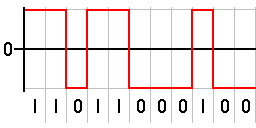
\includegraphics[width=0.7\textwidth]{images/SiSPI/NRZcode.png}

Является простейшим кодом и представляет собой обычный цифровой сигнал. Логическому нулю соответствует низкий уровень сигнала в пределах битового интервала, а логической единице --- высокий.

10 Мб/с -> 1010 - 5 МГц. От 0 до 5 МГц.

Достоинства:
\begin{itemize}
\item нет необходимости использовать дополнительное оборудование для  передачи;
\item низкая требуемая полоса пропускания кабеля.
\end{itemize}

Недостатки:
\begin{itemize}
\item обнаружить передачу при передаче большой последовательности нулей невозможно;
\item невозможность передавать длинные последовательности из-за рассинхронизации передатчика и приёмника.
\item из-за наличия постоянной составляющей в коде невозможно обеспечить гальваническую развязку устройств и линий связи с помощью трансформатора.
\end{itemize}
\subsubsection{RZ}
\label{sec-4_7_2}


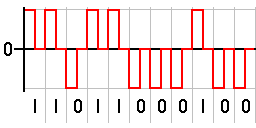
\includegraphics[width=0.7\textwidth]{images/SiSPI/RZcode.png}

Трёхуровневый код, в котором каждый битовый интервал разбивается на два отрезка. В первой половине передаётся значащий уровень сигнала, а во второй половине нулевой. Логическому нулю соответствует положительный переход с низкого на высокий, логической единице отрицательный.

10 Мб/с -> 10 МГц.

Достоинства:
\begin{itemize}
\item код самосинхронизирующийся. По переходу в центре бита синхронизируются приёмник и передатчик;
\item отсутствует постоянная составляющая.
\end{itemize}

Недостатки:
\begin{itemize}
\item три уровня;
\item сложность оборудования;
\item большая требуемая полоса пропускания.
\end{itemize}

Такой можно использовать в оптоволоконных сетях из-за того, что уровень там довольно постоянный, причём высокому уровню соответствует сильный свет, нулевому средний свет, низкому отсутствие света.
\subsubsection{MII}
\label{sec-4_7_3}


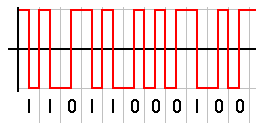
\includegraphics[width=0.7\textwidth]{images/SiSPI/Manchester_code.png}
TODO Картинку проверить

Двухуровневый код. Внутри каждого битового интервала присутствует переход. Логическому нулю соответствует положительный переход, логической единице отрицательный.

10 Мб/с -> 111, 000 - 10 МГц. 101 - 5 МГц.

Достоинства:
\begin{itemize}
\item самосинхронизирующийся двухуровневый код;
\item 2 полосовых фильтра на 5 и 10 МГц отфильтровывают помехи постоянной составляющей в канале;
\item для определения занятости канала необходимо контролировать несущую в течение одного битового интервала;
\item для гальванической развязки можно использовать импульсный трансформатор.
\end{itemize}

Недостатки:
\begin{itemize}
\item большая требуемая полоса частот.
\end{itemize}
\subsubsection{Разностный манчестер}
\label{sec-4_7_4}


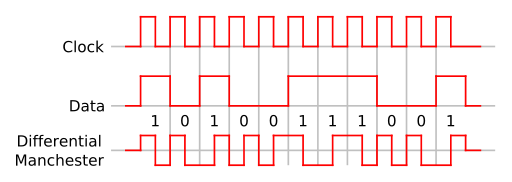
\includegraphics[width=0.7\textwidth]{images/SiSPI/Differential_manchester_encoding.png}

Значение бита определяется по наличию перехода в начале битового интервала. Логический ноль --- переход в начале есть, логическая единица --- перехода в начале нет. В центре битового интервала переход есть всегда.

В современных сетях со скоростями 100 Мб и выше главным требованием к коду является малая полоса пропускания. Поэтому в таких сетях используются разновидности кода NRZ --- MLT3, NRZi и дополнительные кодовые преобразования 4B/5B.

MLT3 --- трёхуровневый код, в котором ноль повторяет предыдущее состояние среды, а единица изменяет состояние среды по следующему закону +U 0, -U 0.

Узнать про MLT3, NRZi и дополнительные кодовые преобразования 4B/5B (62B/64B).
\subsection{Разновидности оборудования локальных телекоммуникационных систем}
\label{sec-4_8}
\subsubsection{Повторитель (repeater)}
\label{sec-4_8_1}


При передаче сигнала по кабелю сигнал испытывает затухание. Для увеличения длины сегмента используются промежуточные усилители сигнала, называемые репиторы.

\emph{Репитор} --- двехпортовое устройство, которое принимает сигнал из одного порта, усиливает его и отправляет в другой свой порт.

Повторитель функционирует только на физическом уровне, не умеет читать данные канального уровня и выше. Следовательно не может осуществлять фильтрацию передаваемых кадров.

Повторитель формирует единую область коллизий или общую среду передачи из всех подключённых к нему сегментов.

Для сети 10 Мб/с = 4, 100 Мб/с = 1.
\subsubsection{Концентратор (hub)}
\label{sec-4_8_2}


\emph{Хаб} (многопортовый повторитель) --- многопортовое устройство, выполняющее роль центрального звена в сети с топологией звезда, построенной на витой паре.

Принимает сигнал из одного порта, усиливает его и отправляет во все остальные порты.

Работает на физическом уровне, формирует единую область коллизий для всех подключённых к нему сегментов.
\begin{itemize}

\item Исполнение концентраторов\\
\label{sec-4_8_2_1}%
\begin{enumerate}
\item Автономные концентраторы. Используются для формирования небольших сетей до 16 портов. Возможно отсутствует порт для соединения с другими концентраторами.
\item Наращиваемые концентраторы. Имеют возможность для соединения нескольких концентраторов друг с другом с помощью специального порта и специального короткого кабеля. Полученное устройство работает как один большой концентратор.
\item Модульные концентраторы. Представляют собой шасси, которые содержат несколько слотов для подключения отдельных портов. Шасси предоставляет для всех общий для всех источник питания и шину для взаимодействия. При этом модули могут относиться к сетям, построенным по различным технологиям.
\end{enumerate}


\item Дополнительные функции концентраторов\\
\label{sec-4_8_2_2}%
Если концентратор функционирует на канальном уровне и может читать заголовки протокола канального уровня, он имеет следующие возможности:
\begin{enumerate}
\item Защита от несанкционированного подключения к порту путём привязки конкретного MAC-адреса к конкретному порту. Возможность принудительного отключения неиспользуемых портов.
\item Отключение неправильно работающих сегментов. Ошибки, которые можно контролировать:

\begin{itemize}
\item связанные с длиной кадра 64\ldots{}1518;
\item неверная контрольная сумма кадра, либо неправильно оформленный заголовок кадра;
\item множественные коллизии. Если порта стал источником столкновения пакетов 60 раз подряд, его отключают;
\item затянувшаяся передача. Если кадр передаётся дольше кадра максимальной длины в 3 раза;
\end{itemize}

\item Поддержка резервных связей.
\item Управление по протоколу SNMP.
\end{enumerate}

\end{itemize} % ends low level
\subsubsection{Мост (bridge)}
\label{sec-4_8_3}


\emph{Мост} --- многопортовое устройство (друхпортовое), работающее на канальном уровне и способное разделять единую область коллизий подключённых к нему сегментов.

Мост принимает кадр из одного порта и определяет местоположение получателя этого кадра. 

Если получатель расположен в другом сегменте, мост передаёт кадр в этот сегмент. Если получатель находится в том же сегменте, что и отравитель, пакет уничтожается.

Обычные режим работы моста называется \emph{прозрачный режим}, т.е. он не имеет собственного MAC-адреса и для сетевых устройств невидим, при этом абоненты подключённых к мосту сегментов могут одновременно передавать кадры без возможных коллизий.

Основным недостатком моста является не поддержка петлевых или кольцевых топологий сетей.

Варианты исполнения мостов:
\begin{enumerate}
\item Прозрачный мост. Объединяет сегменты, построенные по одинаковым технологиям. Никакого перекодирования кадра не происходит внутри порта, возможно работать без полной буферизации кадра, т. е. напрямую.
\item Преобразующий мост. Объединяет сегменты, построенные по разным технологиям. Принимает полностью кадр в буфер, присваивает ему новый заголовок канального уровня и отправляет в соответствующий сегмент.
\item Удалённый мост. Пара удалённых мостов может организовать соединение двух локальных сетей через глобальную сеть. Основной задачей является согласование высокой скорости локальной сети с низкой скоростью глобальной через:

\begin{itemize}
\item большой объём буфера;
\item сжатие трафика;
\item принудительное дублирование служебного трафика.
\end{itemize}

\end{enumerate}
\subsubsection{Коммутатор (switch)}
\label{sec-4_8_4}


\emph{Коммутатор} --- многопортовое устройство, выполняющее роль центрального звена в сети с топологией звезда и функционирующее следующим образом.

Кадр принимается из одного порта и отправляется в порт, к которому подключён получатель. При этом коммутатор может обеспечивать несколько соединений пар портов.

Любое соединение коммутаторов двух портов аналогично выделенному соединению точка-точка и обеспечивается максимальной пропускной способностью сети.
\begin{itemize}

\item Конструкции коммутаторов\\
\label{sec-4_8_4_1}%
Каждый порт коммутатора обслуживает собственный процессор, называемый EPP (ethernet port processor). Координирует работу всех процессоров системный модуль, в котором есть дополнительный процессор --- центральный и коммутационная матрица, в которой хранятся соответствия MAC-адресов и портов.

Коммутационная матрица формируется динамически в процессе работы коммутатора, т. е. при начальном включении коммутатор работает как хаб.

Объединение процессоров возможно тремя способами:
\begin{enumerate}
\item Использование коммутационной матрицы. Каждому кадру при поступлении в коммутатор присваивается т. н. тег --- это комбинация бит, которая определяет адрес порта назначения. Такая матрица реализуется в виде микросхемы и наибольшее распространение получила матрица с 3 уровнями вентилей.
\item Использование внутренней высокоскоростной шины. Используется общая шина с разделением времени.
\item Использование разделяемой памяти.
\end{enumerate}


\item Дополнительные функции коммутаторов\\
\label{sec-4_8_4_2}%
Существует 2 разновидности коммутаторов:
\begin{enumerate}
\item На лету (on fly). В этом случае коммутатор передаёт пакет без задержки. При этом дополнительные функции коммутатора не поддерживаются и количество коммутаторов в сети накладывается тоже ограничения, что и на концентраторы.
\item С буферизацией. Могут полностью сохранять кадр во внутренней памяти и дополнительно позволяют выполнять следующие функции:

\begin{itemize}
\item отбрасывание бракованных кадров;
\item поддержка полнодуплексного режима передачи (full duplex). Кадр передаётся по одному кабелю и каждое устройство может исправить принимаемый сигнал, зная передаваемый. При этом скорость обеспечивается до 200 Мб/сек;
\item поддержка виртуальных локальных сетей (VLAN). Позволяет выделить несколько групп портов коммутатора, которые будут изолированы друг от друга. Коммутация между этими группами портов осуществляться не будет. Связь между VLAN может быть организована только с помощью коммутаторов на сетевом уровне. Один порт может входить одновременно в несколько VLANов;
\item поддержка алгоритма покрывающего дерева (spaning tree). Коммутатор запрещает кольцевые топологии, петлевые маршруты и резервные линии. При первоначальном включении коммутаторов с поддержкой покрывающего дерева, они с помощью обмена служебными пакетами автоматически находят все резервные или петлевые связи и строится логическая иерархическая топология поверх существующей. Все связи, которые не вошли в эту топологию объявляются резервными и соответствующие порты закрываются. В случае, если одна из основных связей нарушается, покрывающее дерево строится заново, включая в себя резервные связи;
\item т. к. коммутатор выступает в качестве получателя кадра, ограничение по количеству коммутаторов в сети снимается.
\end{itemize}

\end{enumerate}

Недостатки коммутаторов --- работа с широковещательным трафиком.

\end{itemize} % ends low level
\subsubsection{Маршрутизатор (router)}
\label{sec-4_8_5}


\emph{Шлюз} --- сетевое устройство, имеющее более одного сетевого интерфейса.

\emph{Роутер} --- шлюз, умеющий маршрутизировать сетевые пакеты между сетевыми интерфейсами.

Маршрутизатор функционируем не выше сетевого уровня, следовательно информации, передаваемой протоколом сетевого уровня должно быть достаточно для нахождения получателя пакетов.

Существует 3 алгоритма маршрутизации:
\begin{enumerate}
\item Маршрутизация от источника. В этом случае в маршрутной таблице хранятся сведения о всех промежуточных узлах на пути следования пакетов, либо эта информация передаётся в самом пакете. Используется в статичных сетях, т. е. где количество абонентов фиксировано и связи определены.
\item Одношаговая маршрутизация. В маршрутной таблице хранятся сведения только о следующем маршрутизаторе или о следующем шаге маршрута. Next Gateway.
\item Случайная маршрутизация. Маршрутных таблиц не создаётся, а каждый пакет отправляется в один из подключённых сетевых интерфейсами.
\end{enumerate}

Существует 2 способа формирования маршрутных таблиц:
\begin{enumerate}
\item Статическая маршрутизация. Каждая маршрутная таблица формируется вручную администратором.
\item Динамическая маршрутизация. Маршрутизаторы самостоятельно обмениваются маршрутными таблицами с помощью специальных протоколов --- RIP, OSPF.
\end{enumerate}
\begin{itemize}

\item Дополнительные функции маршрутизаторов\\
\label{sec-4_8_5_1}%
\begin{enumerate}
\item Отбрасывание бракованных сетевых пакетов. Бракованным пакетом считается пакет, у которого закончился TTL (измеряется в hop'ах). Каждый маршрутизатор вычитает из поля TTL единицу.
\item Фрагментация пакетов. Для каждой сети, подключённой к маршрутизатору он определяет MTU (максимально передаваемый блок) и при передаче большого пакета в сеть с маленьким MTU, он фрагментирует его средствами протокола сетевого уровня. Сбор пакета из фрагмента осуществляется у конечного получателя.
\end{enumerate}

Вместо SNMP используется ICMP.

\end{itemize} % ends low level
\section{Канальный уровень в модели OSI}
\label{sec-5}
\subsection{Методы множественного доступа станций к общему каналу}
\label{sec-5_1}


\begin{enumerate}
\item Случайный множественный доступ.

\begin{itemize}
\item бесконтрольный;
\item бесконтрольный с тактированием;
\item множественный с обнаружением передачи (МДОП);
\item множественный с контролем столкновений (МДКС);
\item МДОП/КС
\end{itemize}

\item Детерминированный множественный доступ.

\begin{itemize}
\item синхронное разделение времени;
\item асинхронное разделение времени;
\item передача полномочий.
\end{itemize}

\item Комбинированный множественный доступ.

\begin{itemize}
\item СМД -> ДМД;
\item ДМД -> СМД;
\item гибридный доступ.
\end{itemize}

\end{enumerate}
\subsubsection{Случайный множественный доступ}
\label{sec-5_1_1}


Все станции сети равноправны и каждая станция самостоятельно определяет момент начала передачи.

Достоинства:
\begin{itemize}
\item надёжность;
\item гибкость;
\item открытость.
\end{itemize}

Недостатки: возможное столкновение пакетов.

Достоинства:
\begin{itemize}
\item станции равноправны и независимы друг от друга.
\item надёжность высокая. Алгоритм децентрализован.
\item возможность включения станций в работающую сеть.
\item при низкой загрузке сети высокая пропускная способность.
\end{itemize}

Недостатки:
\begin{itemize}
\item при высокой загрузке сети низкая пропускная способность.
\item отсутствие гарантированного времени доступа в сеть.
\item невозможность приоритетного доступа в сеть.
\end{itemize}
\begin{itemize}

\item Бесконтрольный метод. "Чистая" ALOHA\\
\label{sec-5_1_1_1}%
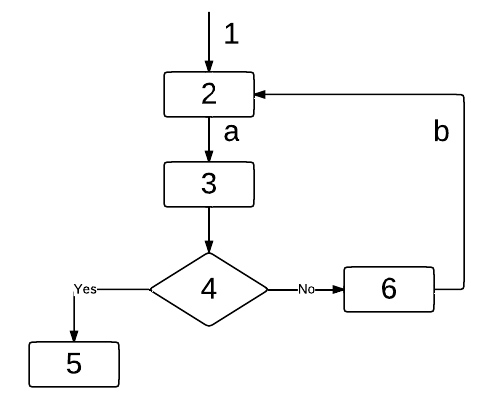
\includegraphics[width=0.7\textwidth]{images/SiSPI/aloha.png}

\begin{enumerate}
\item Необходимость передачи кадра.
\item Станция передаёт кадр.
\item Станция принимает кадр и проверяет на наличие ошибок.
\item Если в кадре ошибка.
\item Ошибок нет. Станция отсылает положительную квитанцию, подтверждающая успешный приём.
\item Ошибки есть. Станция ничего не отсылает. Положение тайм-аут.
\item Необходимость повторной передачи кадра.
\end{enumerate}

При 50\% загрузке сети, количество успешно принятых кадров \~{}18,6\%.


\item Бесконтрольный с тактированием. Синхронная ALOHA\\
\label{sec-5_1_1_2}%
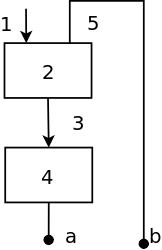
\includegraphics[width=0.7\textwidth]{images/SiSPI/sincaloha.png}

Все станции синхронизированы и начало передачи кадра возможно при получении тактового импульса.

\begin{enumerate}
\item Необходимость передачи кадра.
\item Станция ожидает появления тактового импульса.
\item Станция дождалась появления тактового импульса.
\item Станция передаёт кадр.
\item Необходимость повторной передачи кадра.
\end{enumerate}

Для 50\% загрузки сети количество успешно переданных кадров 37.2\%.


\item Множественный с обнаружением передачи (МДОП)\\
\label{sec-5_1_1_3}%
Станция имеет возможность контролировать занятость канала перед началом передачи.

\begin{enumerate}
\item Необходимость передачи кадра.
\item Станция прослушивает канал.
\item Канал свободен.
\item Станция передаёт кадр.
\end{enumerate}

При 50\% загрузке 80\% успешно переданных кадров.

Существует 3 стратегии поведения станции при контроле занятости канала:
\begin{enumerate}
\item Ненастойчивый МДОП. Если канал свободен, станция сразу передаёт кадр. Если канал занят, станция откладывает повторную проверку канала на определённый или случайный промежуток времени.
\item 1-настойчивый МДОП. Если канала занят, станция настойчиво ждёт его освобождения, после чего с вероятностью 1 передаёт кадр. Если освобождения канал ждут несколько станций вероятностью столкновения 1.
\item p-настойчивый МДОП. Станция настойчиво ждёт освобождения канала, после чего с вероятностью p передаёт кадр в канал. Изменяя значение p, в зависимости от загрузки сети, можно добиться приемлемых показателей вероятности столкновения кадров.
\end{enumerate}


\item Множественный достоинства с контролем столкновений (МДКС)\\
\label{sec-5_1_1_4}%
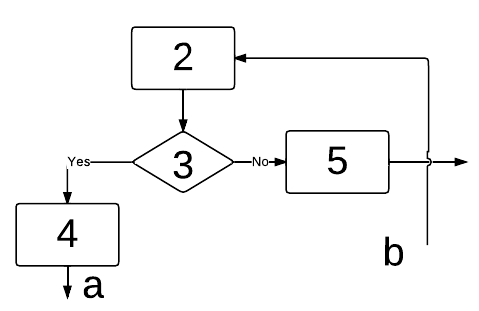
\includegraphics[width=0.7\textwidth]{images/SiSPI/mdks.png}

Станция имеет возможность контролировать канал во время передачи своего кадра. Если передаваемые значения битов не совпадают с принимаемыми из канала, считается, что произошло столкновение.

\begin{enumerate}
\item Необходимость передачи кадра.
\item Станция передаёт кадр и прослушивает канал.
\item Условие. Обнаружено ли столкновение в канале.
\item Столкновения нет. Кадр передаётся до конца.
\item Столкновения есть. Станция прерывает передачу кадра.
\item Необходимость повторной передачи.
\end{enumerate}

\end{itemize} % ends low level
\subsubsection{Детерминированные методы доступа}
\label{sec-5_1_2}
\begin{itemize}

\item Синхронное разделение времени\\
\label{sec-5_1_2_1}%
Время работы сети циклически делится на число интервалов соответствующих числу станций подключённых к каналу. Каждой станции во время цикла предоставляется интервал времени, в течение которого она может использовать канал для передачи кадров. Если станции нечего передавать, его интервал не используется.


\item Асинхронное разделение времени\\
\label{sec-5_1_2_2}%
Каждая станция в цикле получает различный интервал времени для передачи, размер которого определяется либо статистически по загруженности станций, либо размер определяется запрашиваемым и оплаченным станцией сервером.

Достоинства методов разделения времени:
\begin{itemize}
\item нет столкновений;
\item при 100\% загруженности сети пропускная способность канала будет использоваться полностью;
\item гарантированное время доступа в сеть;
\item возможность приоритетного доступа в сеть.
\end{itemize}

Недостатки:
\begin{itemize}
\item неэффективно используется пропускная способность при неполной загрузке;
\item низкая надёжность из-за наличия диспетчера.
\end{itemize}


\item Метод передачи полномочий\\
\label{sec-5_1_2_3}%
В сети циркулирует специальный пакет, который даёт станции полномочия на передачу кадров в канал.

Если станция получает полномочия, она передаёт разрешённое количество кадров в канал, а затем отдаёт полномочия следующей станции. Если станции нечего передавать, она сразу расстаётся с полномочиями.

Достоинства:
\begin{itemize}
\item более эффективное использование пропускной способности;
\item повышается надёжность из-за отсутствия диспетчера;
\item возможна приоритетная передача.
\end{itemize}

Недостатки:
\begin{itemize}
\item возможность потери или дублирования полномочий;
\item низкая гибкость и открытость сети.
\end{itemize}

\end{itemize} % ends low level
\subsubsection{Комбинированные методы доступа}
\label{sec-5_1_3}


Сочетают достоинства случайных и детерминированных методов доступа, т. е. при низкой загрузке сети преимущественно используется случайный множественный доступ, а при высокой детерминированный.
\begin{itemize}

\item Детерминированный доступ с переходом в случайный\\
\label{sec-5_1_3_1}%
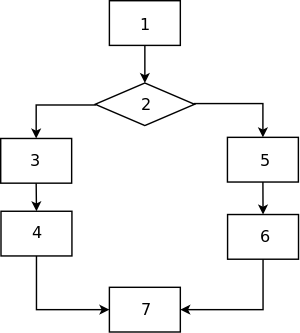
\includegraphics[width=0.7\textwidth]{images/SiSPI/ds.png}

Каждой станции циклически предоставляется временное окно для передачи. Каждое окно состоит из 2 интервалов:
\begin{itemize}
\item интервал управления;
\item интервал передачи.
\end{itemize}

Алгоритм:
\begin{enumerate}
\item Временное окно получило i станция.
\item Есть ли кадр для передачи.
\item В интервал управления станция передаёт служебный кадр о занятости окна.
\item В интервал передачи станция передаёт кадр.
\item Если у станции нет кадра. Станция молчит в интервале управления.
\item Между остальными станциями реализуется СМД в интервал передачи.
\item Временное окно получает i+1 станция.
\end{enumerate}


\item Случайный доступ с переходом в детерминированный\\
\label{sec-5_1_3_2}%
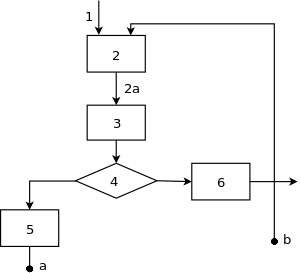
\includegraphics[width=0.7\textwidth]{images/SiSPI/mdopks.png}

Между станциями реализуется МДОП/КС, при этом в цепи циркулируют полномочия, которые получает каждая станция.

\begin{enumerate}
\item Полномочия получает i станция.
\item Есть ли кадр для передачи.
\item Станция передаёт кадр, контролируя столкновения.
\item Есть ли столкновение.
\item Все станции-участники столкновения прекращают передачу кадров.
\item Станция, имеющая полномочия возобновляет передачу кадра и доводит её до конца.
\item Реализуется обычное равноправное МДОП/КС между станциями.
\item Полномочия передаются i+1 станции.
\end{enumerate}

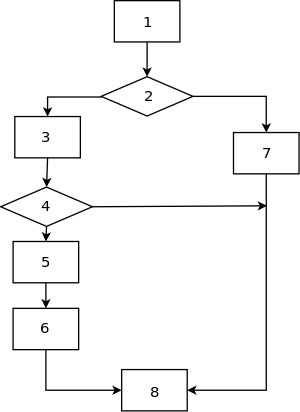
\includegraphics[width=0.7\textwidth]{images/SiSPI/sd.png}


\item Гибридный доступ\\
\label{sec-5_1_3_3}%
В канале существуют средства измерения загрузки. При малой загрузке используется случайный множественный доступ, при большой детерминированный.

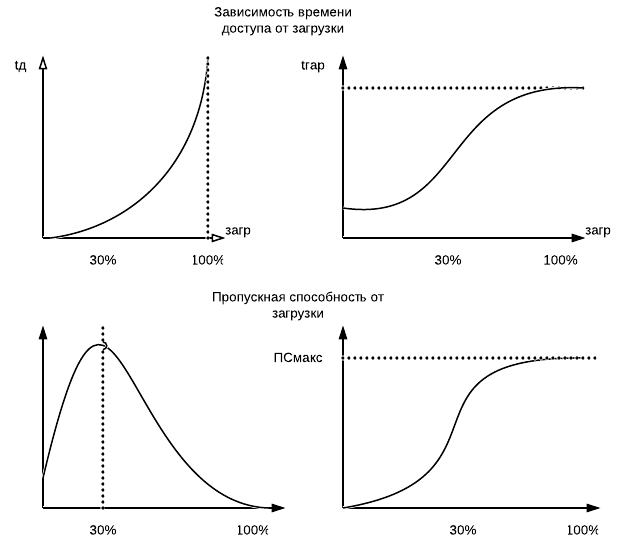
\includegraphics[width=0.7\textwidth]{images/SiSPI/time.png}

\end{itemize} % ends low level
\subsection{Стандарт IEEE 802}
\label{sec-5_2}


Спецификации стандарта IEEE 802 определяют основные параметры для физических компонентов в сети, таких как, сетевая карта NIC (network interface card) и сетевой среды network media. Они определяют механизмы доступа к каналу связи и способы передачи данных.

Особенностью стандарта IEEE 802 является то, что канальный уровень модели OSI представлен в виде 2-х подуровней: LLC и MAC.

\textbf{LLC} подуровень управления логической связью. Функции:
\begin{enumerate}
\item Установление и завершение соединения.
\item Управление потоком кадров.
\item Подтверждение правильности приёма кадров.
\end{enumerate}

Реализуется в виде программного модуля (драйвер сетевой карты) и уровень является общим для нескольких сетевых технологий.

\textbf{MAC} подуровень доступа к среде. Функции:
\begin{enumerate}
\item Управление доступом в передающей среде.
\item Определение границ кадров.
\item Проверка ошибок в кадрах.
\item Распознавание адресов.
\end{enumerate}

MAC уровень реализуется в виде аппаратных компонентов. MAC подуровень уникален для каждой сетевой технологии.

Стандарт IEEE 802 включает следующие разделы:
\begin{enumerate}
\item 802.1 Internet working. Объединение сетей.

\begin{itemize}
\item содержит обзор проекта 802;
\item определяет механизм управления сетью на MAC подуровнях;
\item задаёт требования к локальным сетям;
\end{itemize}

\item 802.2 LLC. Определяет функционирование подуровня LLC.
\item 802.3 Ethernet. Описывает протокол Ethernet и в частности метода доступа CSMA/CD (МДОК/КС).
\item 802.4 Tokken Bus. Сеть с топологией типа шина, используемая в качестве метода доступа передачу полномочий.
\item 802.5 Token Ring. Сеть с передачей полномочий с топологией кольцо.
\item 802.6 MAN. Рекомендации по построению городских сетевой (DQDB).
\item 802.7 Broadband. Технологическая группа по широковещательной передаче. Содержит рекомендации по широкополосным сетевым технологиям, оборудованию и т. д.
\item 802.8 Содержит рекомендации по применению оптоволоконных линий для передачи данных и в частности по их применению в сетях 802.3--802.6. FDDI.
\item 802.9 Технология интегрированной передачи голоса и данных по одной линии. ISDN.
\item 802.10 Network security. В нём рассмотрена безопасность сетей.
\item 802.11 Wireless network. Технология беспроводной передачи данных.
\item 802.12 100VGAnyLAN. Сеть передающая данные на скорости 100Мб на оптоволокне.
\end{enumerate}
\subsubsection{IEEE 802.3 Ethernet}
\label{sec-5_2_1}


В основе механизма доступа Ethernet лежит технология CSMA/CD. 

Все станции равноправны и любая станция может начать передачу, если канал свободен. Занятость канала проверяется по отсутствию несущей в течении 9,6 мкс (межкадровый интервал).

Если канал свободен, станция передаёт кадр и одновременно контролирует наличие столкновений. Если столкновение обнаружено, станция продолжает передачу в течении 32 бит (сигнал jam ``затор'').

Сигнал затора гарантирует, что все станции, участвующие в конфликте гарантированно распознают столкновение. Станция прерывает передачу и возобновляет попытки проверки занят ли канал через случайный промежуток времени, кратный 51,2 мкс, но не более 52 мс. Счётчик попыток станция увеличивает на единицу. Если в течении 16 попыток подряд кадр передать не удаётся из-за коллизий, попытки передачи прекращаются и пользователю передаётся сообщение о невозможности передачи.

При 30\% загрузке сети алгоритм эффективен.
\begin{itemize}

\item Стандарт Fast Ethernet\\
\label{sec-5_2_1_1}%
В начале 90-х годов скорость 10 Мб/сек была недостаточна, была создана рабочая группа, которая начала разрабатывать стандарты построения 100 Мб сети.

В итоге было разработано 3 варианта построения сети, которые вошли в часть 802.3u:
\begin{enumerate}
\item 100BaseTX представлял собой развитие 10BaseT. Сохранял стандартную топологию, формат кадра, но требовался кабель 5-ой категории. Необходимость использования другого способа кодирования --- ?? PAM5, 5-уровневый код, который использует двухбитовое кодирование (\emph{используется в Gigabite Ethernet}).
\item 100BaseT4. Разработан специально для сетей, в которых использовалась витая пара 3-ей категории. Было принято решение использовать для передачи данных в одну сторону все 4 пары кабеля UTP, однако, возникало большое количество искажений сигнала из-за перекрёстных наводок. Для уменьшения количества ошибок одну пару кабеля стали использовать для управления и контроля коллизий. Для передачи данных использовался специальный метод предварительного кодирования 8B/6T. 8 бит исходных данных заменялись 6 троичными символами. В результате символьная скорость для каждой витой пары составляла 25 Мбод, что удовлетворяло требованиям полосы пропускания. Ей соответствует 33,3 Мб/с.
\item 100BaseFX. Стандарт использующий одномодовое оптоволокно. Длина сегмента до 10 километров. Одно волокно используется для передачи, одно для приёма. Разновидности:

\begin{itemize}
\item 100BaseFX WDM. Использует одномодовое одножильное оптоволокно, работающее в режиме full-duplex. Передача и приём одновременно на разных длинах волны. Длина сегмента до 15 км.
\item 100BaseSX. Использует многомодовое оптоволокно и длина сегмента от 300 до 400 метров.
\end{itemize}

\end{enumerate}


\item Стандарт Gigabit Ethernet.\\
\label{sec-5_2_1_2}%
802.3 ab
\begin{enumerate}
\item 1000BaseT. Использует витую пару категории 5E. При передаче используются все 4 пары. Метод кодирования PAM5. Частота гармоники 67.5 Мгц. Длина сегмента 100 м.
\item 1000BaseTX. Использует витую пару 6 категории. Приём и передача осуществляется по одной паре проводов. Длина сегмента до 100 метров.
\item 802.3z.

\begin{itemize}
\item 1000BaseSX. Оптоволокно, длина сегмента 550 метров.
\item 1000BaseSX. Одномодовое оптоволокно для сегмента до 5 км.
\item 1000BaseLH. Одномодовое оптоволокно. Длина сегмента без повторителей --- 100 км.
\item 1000BaseCX. Использует медный твинаксиальный кабель. Длина сегмента до 25 метров.
\end{itemize}

\end{enumerate}


\item Стандарт 10 Gigabit Ethernet.\\
\label{sec-5_2_1_3}%
802.3 ae
\begin{enumerate}
\item 10GBaseCX4. Используется медный кабель типа CX4. Длина сегмента до 15 метров.
\item 10GBaseSR. Используется многомодовое оптоволокно. Длина сегмента до 82 метров.
\item 10GBaseLX4. Используется многомодовое оптоволокно с предварительным уплотнением сигнала по длине волны. Длина сегмента до 300 метров.
\item 10GBaseLR/ER. Одномодовое оптоволокно. Длина сегмента от 10 до 40 км.
\item 10GBaseSW. Используются для формирования каналов STM-64 синхронной цифровой иерархии и имеет соответствующий физический интерфейс.
\item 10GBaseLW.
\item 10GBaseEW.
\end{enumerate}

802.3 an
10GBaseT. Использует экранированную витую пару 6 или выше категории. Длина сегмента 100 м. 

\end{itemize} % ends low level
\subsubsection{Сеть 802.8 FDDI}
\label{sec-5_2_2}


ANSI X3T9.5.

Сеть была разработана 1985 году. Являлся развитием сети Token Ring (802.5).

Топология сети --- кольцо (двойное кольцо). Скорость передачи данных 100 Мб/с. Максимальное количество станций --- 1000. Максимальная длина кольца --- 20 км. Максимальное расстояние между 2-мя станциями --- 2 км. Максимальная длина кадра 4500 байт.
\begin{itemize}

\item Особенности топологии\\
\label{sec-5_2_2_1}%
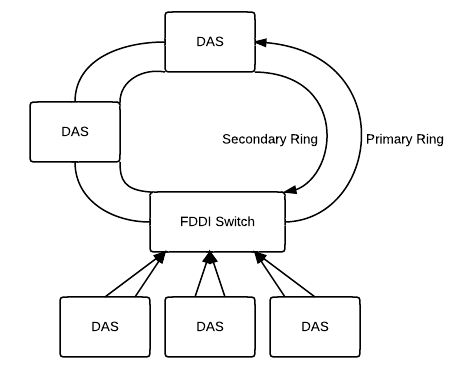
\includegraphics[width=0.7\textwidth]{images/SiSPI/fddi.png}

Топология сети --- двойное кольцо, данные по которым передаются в противоположных направлениях. Одно кольцо --- первичное (primary), второе кольцо --- вторичное (secondary) находится в резерве.

Станции бывают двух видов:
\begin{enumerate}
\item Станции DA (dual-attachment) с повышенными требованиями по надёжности. Подключены и к первичным, и к вторичным кольцам.
\item Станции SA (single-attachment) с обычными требованиями по надёжности. Подключены только к первичному кольцу.
\end{enumerate}

Режимы работы:
\begin{enumerate}
\item Нормальный. Если все узлы функционируют правильно, данные передаются только по первичному кольцу. Вторичное может быть задействовано только в режиме full duplex.
\item Сворачивание кольца. Если выходит из строя узел или линия связи, то адаптеры, ближайшие к месту аварии объединяют первичное и вторичное кольцо, т. к. кольца разнонаправлены, данные продолжают циркулировать между узлами и топология кольцо сохраняется.
\end{enumerate}


\item Метод доступа\\
\label{sec-5_2_2_2}%
По кольцу циркулирует специальный кадр, называемый маркер доступа или token доступа. Когда станция получает маркер, она задерживает его на определённое время (THT) и передаёт кадры в кольцо. По истечении времени THT станция заканчивает передачу последнего кадра и следом за ним отправляет маркер следующей станции.

Кадры последовательно проходят через каждую станцию сети. Если станция распознала адрес получателя как свой, она принимает кадр, проверяет ошибки и устанавливает в заголовке кадра 3 флага:
\begin{enumerate}
\item флаг успешного распознавания адреса;
\item флаг успешного копирования в буфер;
\item флаг отсутствия ошибок.
\end{enumerate}

После чего кадр дальше отправляется по кольцу. Станция-источник кадров получает свои кадры, прошедшие полный оборот, изымает их из кольца и по состоянию флагов оценивает успешность передачи.

Если станции нечего передавать, она не задерживает маркер.

Основной недостаток алгоритма --- возможность потери маркера. Для процедуры восстановления таймера используется дополнительный таймер на каждой станции, который считает время оборота маркера (TRT). 

Станция, у которой истекло время оборота маркера, может создать маркер и, не удерживая его на время THT, отправить его дальше в кольцо. При этот у следующей станции THT не истечёт, и она воспользуется новым маркером.

Если станция, создавшая маркер, получает старый маркер из кольца, она его удаляет.


\item Формат кадра FDDI\\
\label{sec-5_2_2_3}%
\begin{center}
\begin{tabular}{rrrllrlll}
  P  &  SD  &  FC  &  SA   &  DA   &  Data  &  CRC  &  ED  &  FS  \\
 16  &   1  &   1  &  2/6  &  2/6  &  4500  &       &      &      \\
\end{tabular}
\end{center}



\begin{enumerate}
\item Преамбула.
\item Стартовый разделитель.
\item Поле управления кадра CLFFZZZZ.

\begin{itemize}
\item C флаг типа кадра. Синхронный или асинхронный.
\item L флаг длины адреса кадра. MAC или внутренний адрес 2 байта.
\item FF флаг, определяющий тип данных. Либо пользовательские, либо служебные.
\item Z детализирует тип служебного кадра.
\end{itemize}

\item FS поле статуса. ACS00000.

\begin{itemize}
\item A флаг распознавания адреса.
\item C флаг успешного копирования в буфер.
\item S флаг отсутствия в кадре ошибок.
\end{itemize}

\end{enumerate}


\item Стек протоколов FDDI\\
\label{sec-5_2_2_4}%
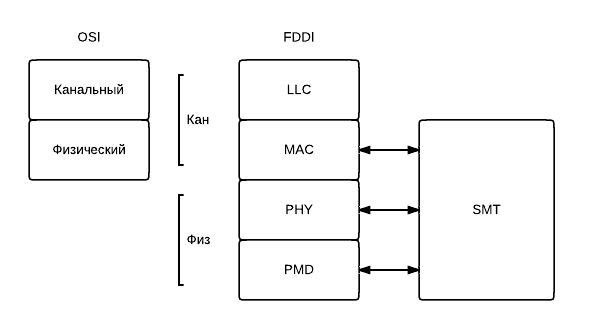
\includegraphics[width=0.7\textwidth]{images/SiSPI/ffdi.png}

\begin{enumerate}
\item PMD. Протокол, зависящий от физической среды. Определяет волоконно-оптический кабель, коннекторы FDDI и оптико-электронный интерфейс.
\item PHY. Физический уровень. Отвечает за синхронизацию приёмника-передатчика, механизм установления тактовой частоты, кодирование декодирование информации, использование кодового преобразования 4B/5B, анализ и обработка служебных символов.
\item MAC подуровень доступа к среде. Управляет доступом станции к среде, управляет процедурой передачи маркера, генерирует CRC и проверяет её, адресует кадры и распознаёт адреса кадров. Удаляет кадры, адресатом которых является.
\item SMD протокол станционного управления. Определяет процедуры управления работой кольца на каждом из уровней. Для каждого уровня существует отдельный набор управляющих сообщений. На уровне PMD они позволяют локализовать неисправность кабеля, на уровне PHY обнаружить неисправные или отключившиеся станции. В обоих случаях управление процедурой сворачивания кольца. На уровне MAC управление восстановлением маркера в случае его потери.
\end{enumerate}


\item Стандарт FFDI2\\
\label{sec-5_2_2_5}%
Основной задачей сети FDDI является надёжная и гарантированная передача данных между узлами. Однако использование этой сети для передачи изохронного трафика (требующий постоянной пропускной способности во времени) неэффективен.

Стандарт FDDI2 обеспечивает улучшенные характеристики по обслуживанию как обычных данных, так и потоковых. Для этого в нём дополнительно используется режим коммутации логических каналов.

Пропускная способность канала 100 Мб/с разбивается на 16 разнесённых по частоте каналов со скоростью 6.144 Мб/с. Каждый из подканалов может быть разделён ещё на несколько подканалов с шагом 8 кб/с. Данные по кольцу передаются в формате цикла, который создаёт главная станция, которая назначается каждый раз при инициализации кольца.

Циклом является последовательность 15625  бит, передаваемая каждые 125 мкс, т.е. 8000 раз в секунду. Для установления изохронного канал между двумя станциями, они обращаются к главной станции по протоколу SMT с заявкой на требуемую пропускную способность. Если в каждом цикле станции будет предоставлен 1 бит для передачи данных, это будет соответствовать выделенному каналу с пропускной способностью 8 кб/с. Если 1 байт, 64 кбит/с.

\end{itemize} % ends low level
\subsubsection{Промышленный стандарт локальных сетей. Модель Pro Way}
\label{sec-5_2_3}


Модель Pro Way разработана для автоматизированных систем управления технологическими процессами.

Модель Pro Way включает 5 уровней:
\begin{enumerate}
\item Прикладной.
\item Сетевой.
\item Магистральный.
\item Канальный.
\item Физический.
\end{enumerate}
\begin{itemize}

\item Физический уровень\\
\label{sec-5_2_3_1}%
Устанавливает правила преобразования кадра из формата, принятого для представления в станциях, в оборудовании и т. д. в единый формат, пригодный для передачи по сети.

Функции:
\begin{itemize}
\item гальваническая развязка цепей, оборудования и ЛС;
\item контроль качества сигнала;
\item синхронизация приёника и передатчика;
\item контроль состояния сети связи (свободна, занята).
\end{itemize}


\item Канальный уровень\\
\label{sec-5_2_3_2}%
Выполняет следующие функции:
\begin{itemize}
\item обнаружение ошибок в заголовке кадра;
\item обнаружение ошибок в данных. Общая вероятность пропуска или принятия ошибочного бита BER = 3*10$^{\mathrm{15}}$.
\item распознавание кадров, адресованных станции.
\end{itemize}

Формат кадра:

\begin{center}
\begin{tabular}{lr}
 Преамбула          &  >1  \\
 Адрес получателя   &   1  \\
 Поле управления    &   1  \\
 Адрес отправителя  &   1  \\
 КС заголовка       &   2  \\
 Данные             &   n  \\
 КС данных          &   2  \\
\end{tabular}
\end{center}



Поле управления:

\begin{center}
\begin{tabular}{lllllll}
 C  &  CA  &  IA  &  I  &  T(2)  &  T  &  R  \\
\end{tabular}
\end{center}



\begin{enumerate}
\item \texttt{С}. Признак командного кадра.
\item \texttt{CA}. Признак подтверждения команды.
\item \texttt{IA}. Признака принятия информационного кадра.
\item \texttt{I}. Признак информационного кадра + \texttt{T(2)} -> команда.
\item \texttt{T}. Номер передаваемого кадра.
\item \texttt{RR}. Номер последнего успешно переданного кадра.
\end{enumerate}

Т. к. для нумерации кадров используется 1 бит, количество неподтверждённых кадров не может превышать одного.


\item Магистральный уровень\\
\label{sec-5_2_3_3}%
Обеспечивает управление доступом станции к каналу. Существует 6 иерархических функций магистрального уровня.

Способность станции выполнять ту или иную функцию называется \emph{статус} станции. Статус может меняться в процессе функционирования сети.

\begin{enumerate}
\item Приём. Станция принимает все правильные кадры, которые ей предназначены, отвечать она на них не может.
\item Исполнение. Кроме приёма станция может послать ответ на ей адресованный кадр.
\item Функция инициации.

\begin{itemize}
\item запросить доступ к магистрали у станции-контролёра;
\item передача кадров станциям-приёмникам;
\item выбор исполнителя для одного шага обмена данными.
\end{itemize}

\item Заказ. Является дополнительным статусов к первым 3-м и позволяет станции изменить свой статус для получения доступа к магистрали ввиду неотложной необходимости (авария).
\item Контроль.

\begin{itemize}
\item управление доступом к каналу путём установления инициатора для каждого шага обмена данными;
\item контроль работы инициаторов;
\item исключение перегрузок, вносимых инициаторами;
\item контроль отказов инициаторов.
\end{itemize}

\item Распоряжение. Станция-распорядитель передаёт управление магистралью путём назначения станции-контролёра и обеспечивает непрерывность управления при её отказе.
\end{enumerate}

В качестве метода доступа используется передача маркера в сети с топологией шина.


\item Сетевой уровень\\
\label{sec-5_2_3_4}%
Если ОСУ ТП(?) состот из из нескольких магистралей, сетевой уровень организует связь между ними.

Управление сетью возлагается на станцию, имеющую статус \emph{директора}, функции которой следующие:
\begin{enumerate}
\item Назначение распорядителей для каждой магистрали.
\item Контроль отказов распорядителей.
\end{enumerate}


\item Прикладной уровень\\
\label{sec-5_2_3_5}%
Обработка данных, получаемых от оператора, технологических процессов, оборудования и т. д.

\end{itemize} % ends low level
\subsubsection{Городские сети (MAN) 802.6}
\label{sec-5_2_4}


Городская сеть занимает промежуточное место между глобальными и локальными сетями и обеспечивает высокоскоростной обмен данными между отдельными компьютерами и локальными сетями в пределах ограниченной территории.

В стандарте 802.6 описывает стандарт построения городской сети на основе протокола SMDS.

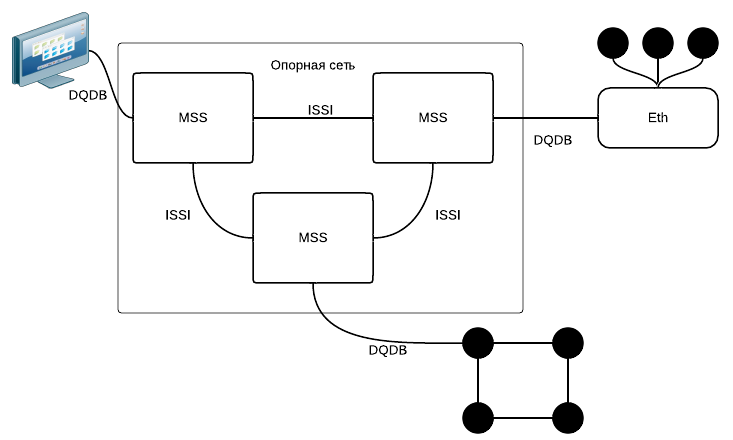
\includegraphics[width=0.7\textwidth]{images/SiSPI/man.png}

Опорная сеть строится на устройствах коммутации (MSS) со специальным интерфейсом между ними (ISSI). Подключение пользователей к подобной сети происходит по протоколу DQDB.
\begin{itemize}

\item Протокол DQDB\\
\label{sec-5_2_4_1}%
В протоколе DQDB определено 2 уровня --- физический и канальный.

\emph{Физический уровень} обеспечивает связь по оптоволоконному или широкополосному медному кабелю между оборудованием пользователя и устройством коммутации со скоростями от 1 до 34 Мбит/с. В качестве топологии используются разнонаправленные шины и каждое устройство подключено к обоим из них.

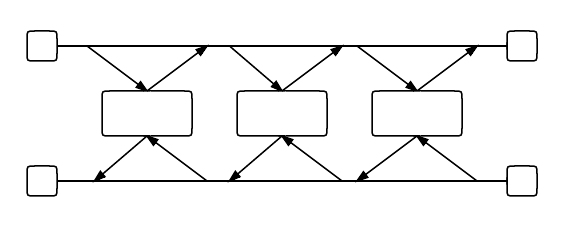
\includegraphics[width=0.7\textwidth]{images/SiSPI/dqdb.png}

На концах на каждой из шин располагается каналообразующее оборудование.

\emph{Канальный уровень}. Данные передаются в виде кадров определённой длины каждые 125 мкс. Формат кадра:

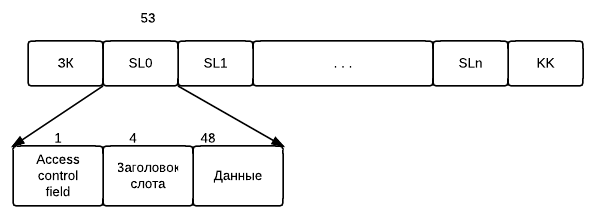
\includegraphics[width=0.7\textwidth]{images/SiSPI/chan.png}

В поле ACF существенными являются 3 флага:
\begin{itemize}
\item признак занятости слота;
\item флаг запроса доступа к каналу;
\item режим работы.
\end{itemize}
  
Режим предопределённой передачи. Каждая станция получает возможность полного или частичного использования поле данных слота. Размер используемого поля данных определяет пропускную способность виртуального канала, который получает станция. В этом режиме в заголовке слота передаётся идентификатор виртуального канала.

Режим случайной передачи. Станции могут использовать слот случайным образом, используя специальный алгоритм распределённой очереди. При этом в заголовке слота устанавливаются все 1.

В зависимости от направления передачи одна шина используется для передачи данных, а другая шина для передачи запросов на доступ к каналу. При этом по шине данных значимым будет флаг \emph{пустой или занятый слот}, а по шине запросов \emph{флаг запросов}.

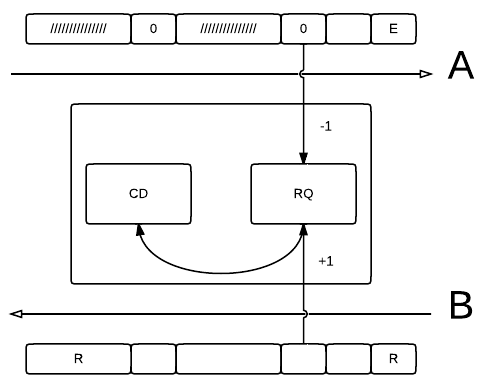
\includegraphics[width=0.7\textwidth]{images/SiSPI/counters.png}

Для передачи в каждую сторону у станции существует 2 типа счётчиков:
\begin{itemize}
\item RQ счётчик запросов.
\item CD декрементный счётчик.
\end{itemize}

Счётчик RQ увеличивается на 1 каждый раз, когда по шине запросов передаётся запрос. Счётчик RQ уменьшается на 1 каждый раз, когда по шине данных передаётся пустой слот.

Если станции необходимо занять слот в шине A, содержимое счётчика RQ передаётся в CD, счётчика RQ обнуляется, а в шину запросов передаётся запрос.

Счётчик CD уменьшается на 1 каждый раз, когда по шине данных передаётся пустой слот. Как только значение счётчика CD достигает 0, станция может использовать первый свободный слот шины A для передачи своих кадров.

\end{itemize} % ends low level
\subsubsection{Технологии глобальных сетей}
\label{sec-5_2_5}


\begin{enumerate}
\item Dial UP. С помощью аналоговых модемов.
\item PDH. Технология плезиохронной цифровой иерархии.
\item SDH/SONet. Синхронная цифровая иерархия.
\item ISDN. Цифровая сеть с интеграцией услуг.
\item xDSL. Цифровая пользовательская линия.
\end{enumerate}
\subsubsection{Аналоговая линия}
\label{sec-5_2_6}


Аналоговая телефонная линия предполагает использование аналоговых модемов, которые передают сигнал в полосе частот 0.3--3.4 кГц. Из-за шумов квантования, возникающих при процедуре АЦП, максимальная скорость передачи данных ограничена 35 кбит/с по теореме Шеннона.

Для двухпроводных линий модемы работают по протоколам серии V (V22 (1200 бит/с)--V34+ (33.6 кбит/с)). V.4x определяют способы помехоустойчивого кодирования, которые улучшают качество связи. V.90 является асинхронным. Скорость нисходящего (56,6 кбит/с), исходящего (33,6 кбит/с).
\subsubsection{Цифровые выделенные линии. Технология PDH}
\label{sec-5_2_7}


В качестве передающей среды используется широкополосный медный кабель, либо оптоволоконный. Оборудование PDH существует двух видов: европейская, американский.


\begin{center}
\begin{tabular}{lrr}
 Канал  &  Количество ТЛФ  &  Скорость, Мб/с  \\
\hline
 E1     &              30  &           2.048  \\
 E2     &             120  &           8.488  \\
 E3     &             480  &          34.368  \\
 E4     &            1920  &         139.264  \\
\end{tabular}
\end{center}



Недостатки технологии PDH --- простой формат кадра на канальном уровне, в котором для каждого телефонного канала выделяется определённый объём данных.

Если телефонный канал не используется, слот заполняется нулями.
Поэтому по прямому назначению технология не используется, а используется в качестве пользовательского варианта подключения к сети, где в кадре передаются данные без привязки к телефонному каналу.
\subsubsection{SDH/SONet}
\label{sec-5_2_8}


Использует более сложный формат кадра, в качестве среды передачи --- оптоволокно и обеспечивает более высокие скорости передачи данных.


\begin{center}
\begin{tabular}{lr}
 Канал  &  Скорость  \\
\hline
 STM1   &   155.520  \\
 STM16  &      2488  \\
\end{tabular}
\end{center}



Т. к. кадр SDH имеет не жёсткую структуру, STM1 позволяет полностью инкапсулировать кадр E4, обеспечивая совместимость технологий.
\subsubsection{ISDN}
\label{sec-5_2_9}


Основная задача ISDN --- передача голосовых и других видов данных (интернет, факс) по обычной телефонной линии.

ISDN предполагает использование следующих разновидностей каналов:


\begin{center}
\begin{tabular}{lll}
 Тип канал  &  Скорость    &  Назначение                         \\
\hline
 A          &  -           &  Выделенная телефонная линия        \\
 B          &  64 кб/с     &  Передача одного голосового канала  \\
 C          &  8/16 кб/с   &  Передача данных                    \\
 D          &  16/64 кб/с  &  Канал управления                   \\
 E          &  64 кб/с     &  Канал внутренней сигнализации      \\
 H0         &  384         &                                     \\
 H10        &  1472        &  Передача                           \\
 H11        &  1536        &  данных                             \\
 H12        &  1920        &                                     \\
\end{tabular}
\end{center}



Для пользователя существует BRI --- базовый пользовательский интерфейс, который включает в себя в себя 2B + D = 144 кб/с.
\subsubsection{xDSL}
\label{sec-5_2_10}


Представляет собой технологию передачи цифровых данных по существующей абонентской сети, в т. ч. и коммутируемой без ограничений использования полосы частот.

Все технологии DSL делятся на 2 вида:
\begin{itemize}
\item синхронные;
\item асинхронные.
\end{itemize}

Синхронные обеспечивают одинаковые скорости исходящего и входящего трафика.

Для асихронных скорость входящего потока выше.


\begin{center}
\begin{tabular}{llrrl}
 Технология       &  Скорость            &      Расстояние  &  ТЛФ пар  &  Назначение         \\
\hline
 ISDL             &  144 кб/с            &             5.5  &        1  &  ISD N              \\
 SDSL             &  2.048 Мб/с          &               3  &        1  &  E1                 \\
 HDSL             &  2.048 Мб/с          &             4.5  &        2  &  E1                 \\
\hline
 ADSL             &  8.0 Мб/с, 1 Мб/с    &             5.5  &        1  &  Inet               \\
 ADSL lite        &  1.5 Мб/с, 0.5 Мб/с  &             5.5  &        1  &  Inet без сплитера  \\
 ADSL 2 Annex J   &  12 Мб/с, 3.5 Мб/с   &             5.5  &        1  &  Inet               \\
 ADSL 2+ Annex M  &  24 Мб/с, 3.5 Мб/с   &             5.5  &        1  &  Inet               \\
\hline
 VDSL             &  65 Мб/с, 1.5 Мб/с   &  300 м (1200 м)  &   Коакс.  &  Телевидение по     \\
                  &                      &                  &           &  запросу            \\
\end{tabular}
\end{center}
\begin{itemize}

\item Спектр ADSL сигнала\\
\label{sec-5_2_10_1}%
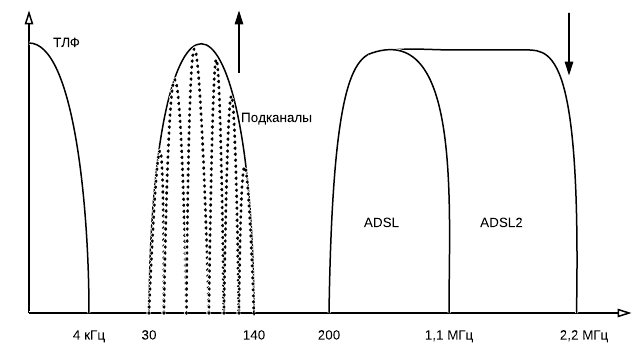
\includegraphics[width=0.7\textwidth]{images/SiSPI/spectr.png}

В случае, когда в канале существует сосредоточенная помеха, часть диапазона, которая затрагивается, исключается из общего спектра сигнала. Скорость при этом уменьшается, но связь остаётся устойчивой.

\end{itemize} % ends low level
\subsubsection{Протоколы канального уровня для выделенных линий}
\label{sec-5_2_11}

\end{document}
